\documentclass[8pt,pdf,hyperref={unicode}]{beamer}
% \documentclass[aspectratio=43]{beamer}
% \documentclass[aspectratio=1610]{beamer}
% \documentclass[aspectratio=169]{beamer}
\usepackage{lmodern}
\usepackage{amsfonts}
\usepackage{amsmath}

\graphicspath{{figures/}}

% тема оформления
%\usetheme{CambridgeUS}
%Закругление выделений
%\useinnertheme{rounded}
%Настройка темы самого слайда
%\useoutertheme{infolines}
%\useoutertheme[subsection=true, footline=authortitle]{miniframes}
\usetheme{Boadilla}
\useoutertheme[subsection=true, footline=authortitle]{miniframes}
\makeatother
\setbeamertemplate{footline}
{
    \leavevmode%
    \hbox{%
        \begin{beamercolorbox}[wd=.4\paperwidth,ht=2.25ex,dp=1ex,center]{author in head/foot}%
            \usebeamerfont{author in head/foot}\insertshortauthor
        \end{beamercolorbox}%
        \begin{beamercolorbox}[wd=.6\paperwidth,ht=2.25ex,dp=1ex,center]{title in head/foot}%
            \usebeamerfont{title in head/foot}\insertshorttitle\hspace*{3em}
            \insertframenumber{} / \inserttotalframenumber\hspace*{1ex}
        \end{beamercolorbox}}%
        \vskip0pt%
    }
\makeatletter
% отключить клавиши навигации
\setbeamertemplate{navigation symbols}{}
% цветовая схема
\usecolortheme{spruce}


\title{ Reactor like TGE model}   
%\subtitle{Overview report}
\author{\underline{Mikhail Zelenyi}\inst{1,2,3} \and Alexandr Nozik\inst{1,2} \and Egor Stadnichuk\inst{1,2}}
\institute[INR]{
    \inst{1} Institute for Nuclear Research of RAS \and
    \inst{2} Moscow Institute of Physics and Technology (NRU)
     \and
	\inst{3} Space Research Institute of RAS }
\date{\today}

%\logo{\includegraphics[height=5mm]{image/logo.png}\vspace{-7pt}}

\begin{document}
    % титульный слайд
    \begin{frame}
        \titlepage
    \end{frame}
%\begin{frame}
%   \frametitle{}
% 
%\end{frame}
%
\begin{frame}
\frametitle{Thunderstorm cloud and lighting: paths for research}

\end{frame}

\begin{frame}
\frametitle{History}
	\begin{columns}
		\begin{column}{0.5\textwidth}
			TGF ---
		\end{column}
		\begin{column}{0.5\textwidth}
			TGE ---
		\end{column}
	\end{columns}
\end{frame}

\begin{frame}
\frametitle{Existing model}
\begin{columns}
\begin{column}{0.5\textwidth}
    \begin{figure}[htb]
        \centering
        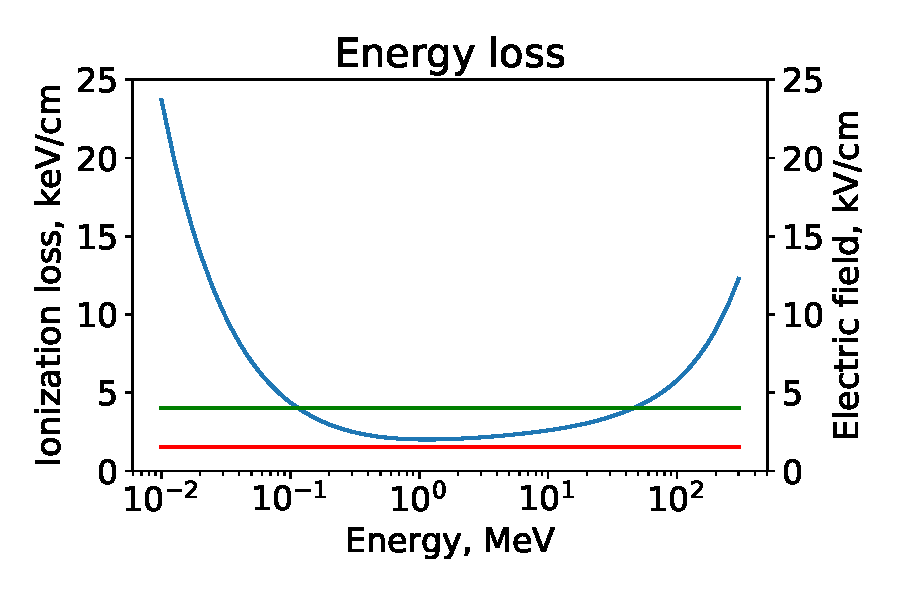
\includegraphics[width=1\columnwidth]{01_Gurevich.pdf}
    \end{figure}
    \textbf{Gurevich model --- Runway breakdown}
\begin{itemize}
    \item Breakdown with help secondary ionization of relativistic electron
    \item If field over MIP loss - run breakdown
\end{itemize}
\end{column}
\begin{column}{0.5\textwidth}
     \textbf{Dwyer model --- Gamma and positron feedback}
    \begin{itemize}
        \item Electron emit bremsstrahlung (including directed to back)
        \item Compton scattering direct gamma to back 
        \item Gamma create new primary electron in top area of cloud
        \item Gamma ray conversion in electron-positron pair
        \item Positron accelerate by field and ionizes cloud creating new primary electron
        
    \end{itemize}
\end{column}
\end{columns}

\end{frame}



\begin{frame}
\frametitle{Disadvantages of existing model}
\begin{itemize}
    \item Gurevich model of runway breakdown don't give ionization for lighting initiation
    \item Dwyer model of feedback don't work in real condition [1]
    \item A long-lasting phenomena as TGE  can't exist in Dwyer model
    \item This models use uniform electric field where as field in cloud have more difficult structure 
\end{itemize}
\small{[1] Calculation of gain coefficient in Dwyer relativistic discharge feedback model of thunderstorm runway breakdown
    EPJ Web of Conferences 201, 07003 (2019), \url{https://doi.org/10.1051/epjconf/201920107003}}
\end{frame}

 % Local background must be enclosed by curly braces for grouping.
\usebackgroundtemplate{
    \hspace*{-2cm}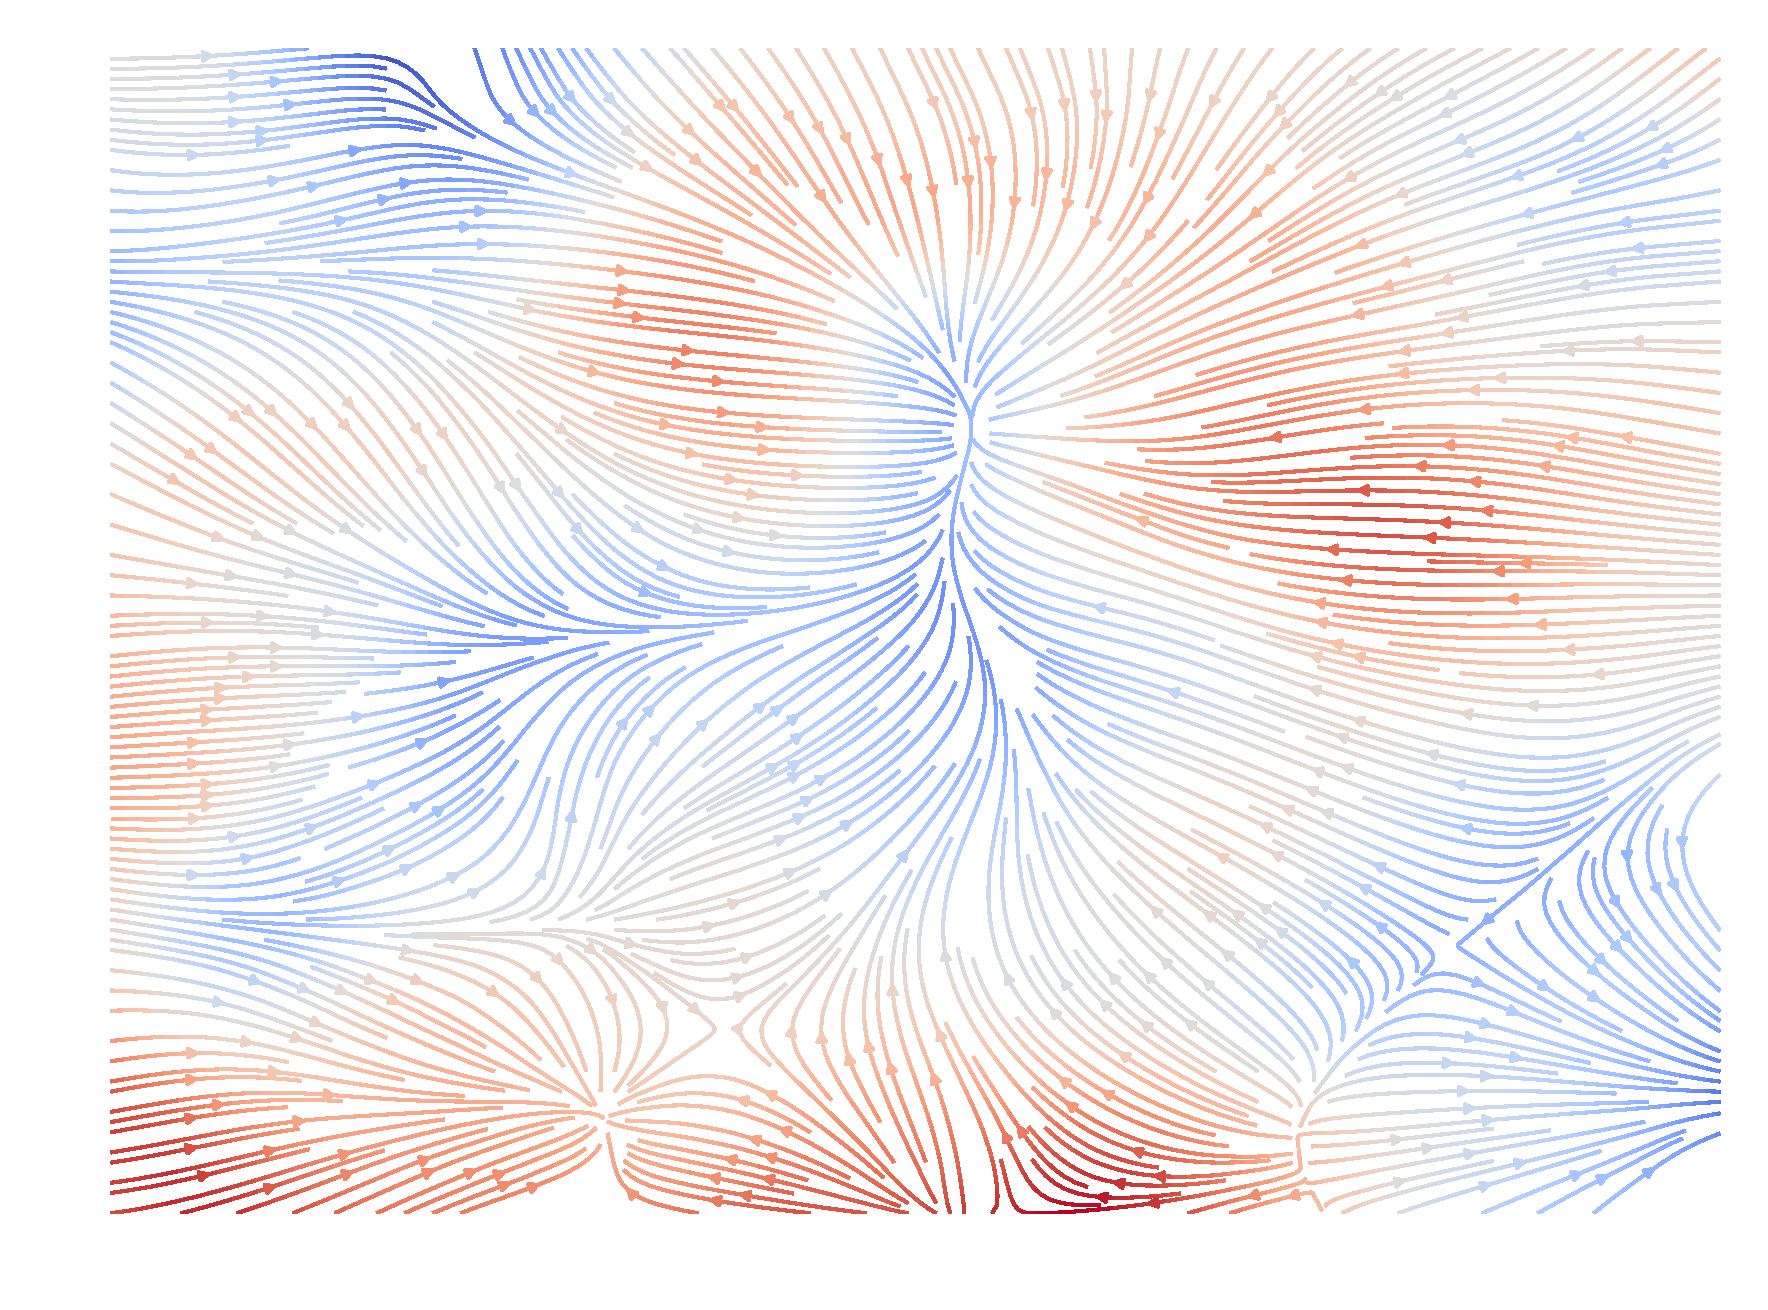
\includegraphics[width=1.2\paperwidth]{electric_streams.pdf}
    
}%
\begin{frame}
    \frametitle{Reactor Like TGE model}
 \centering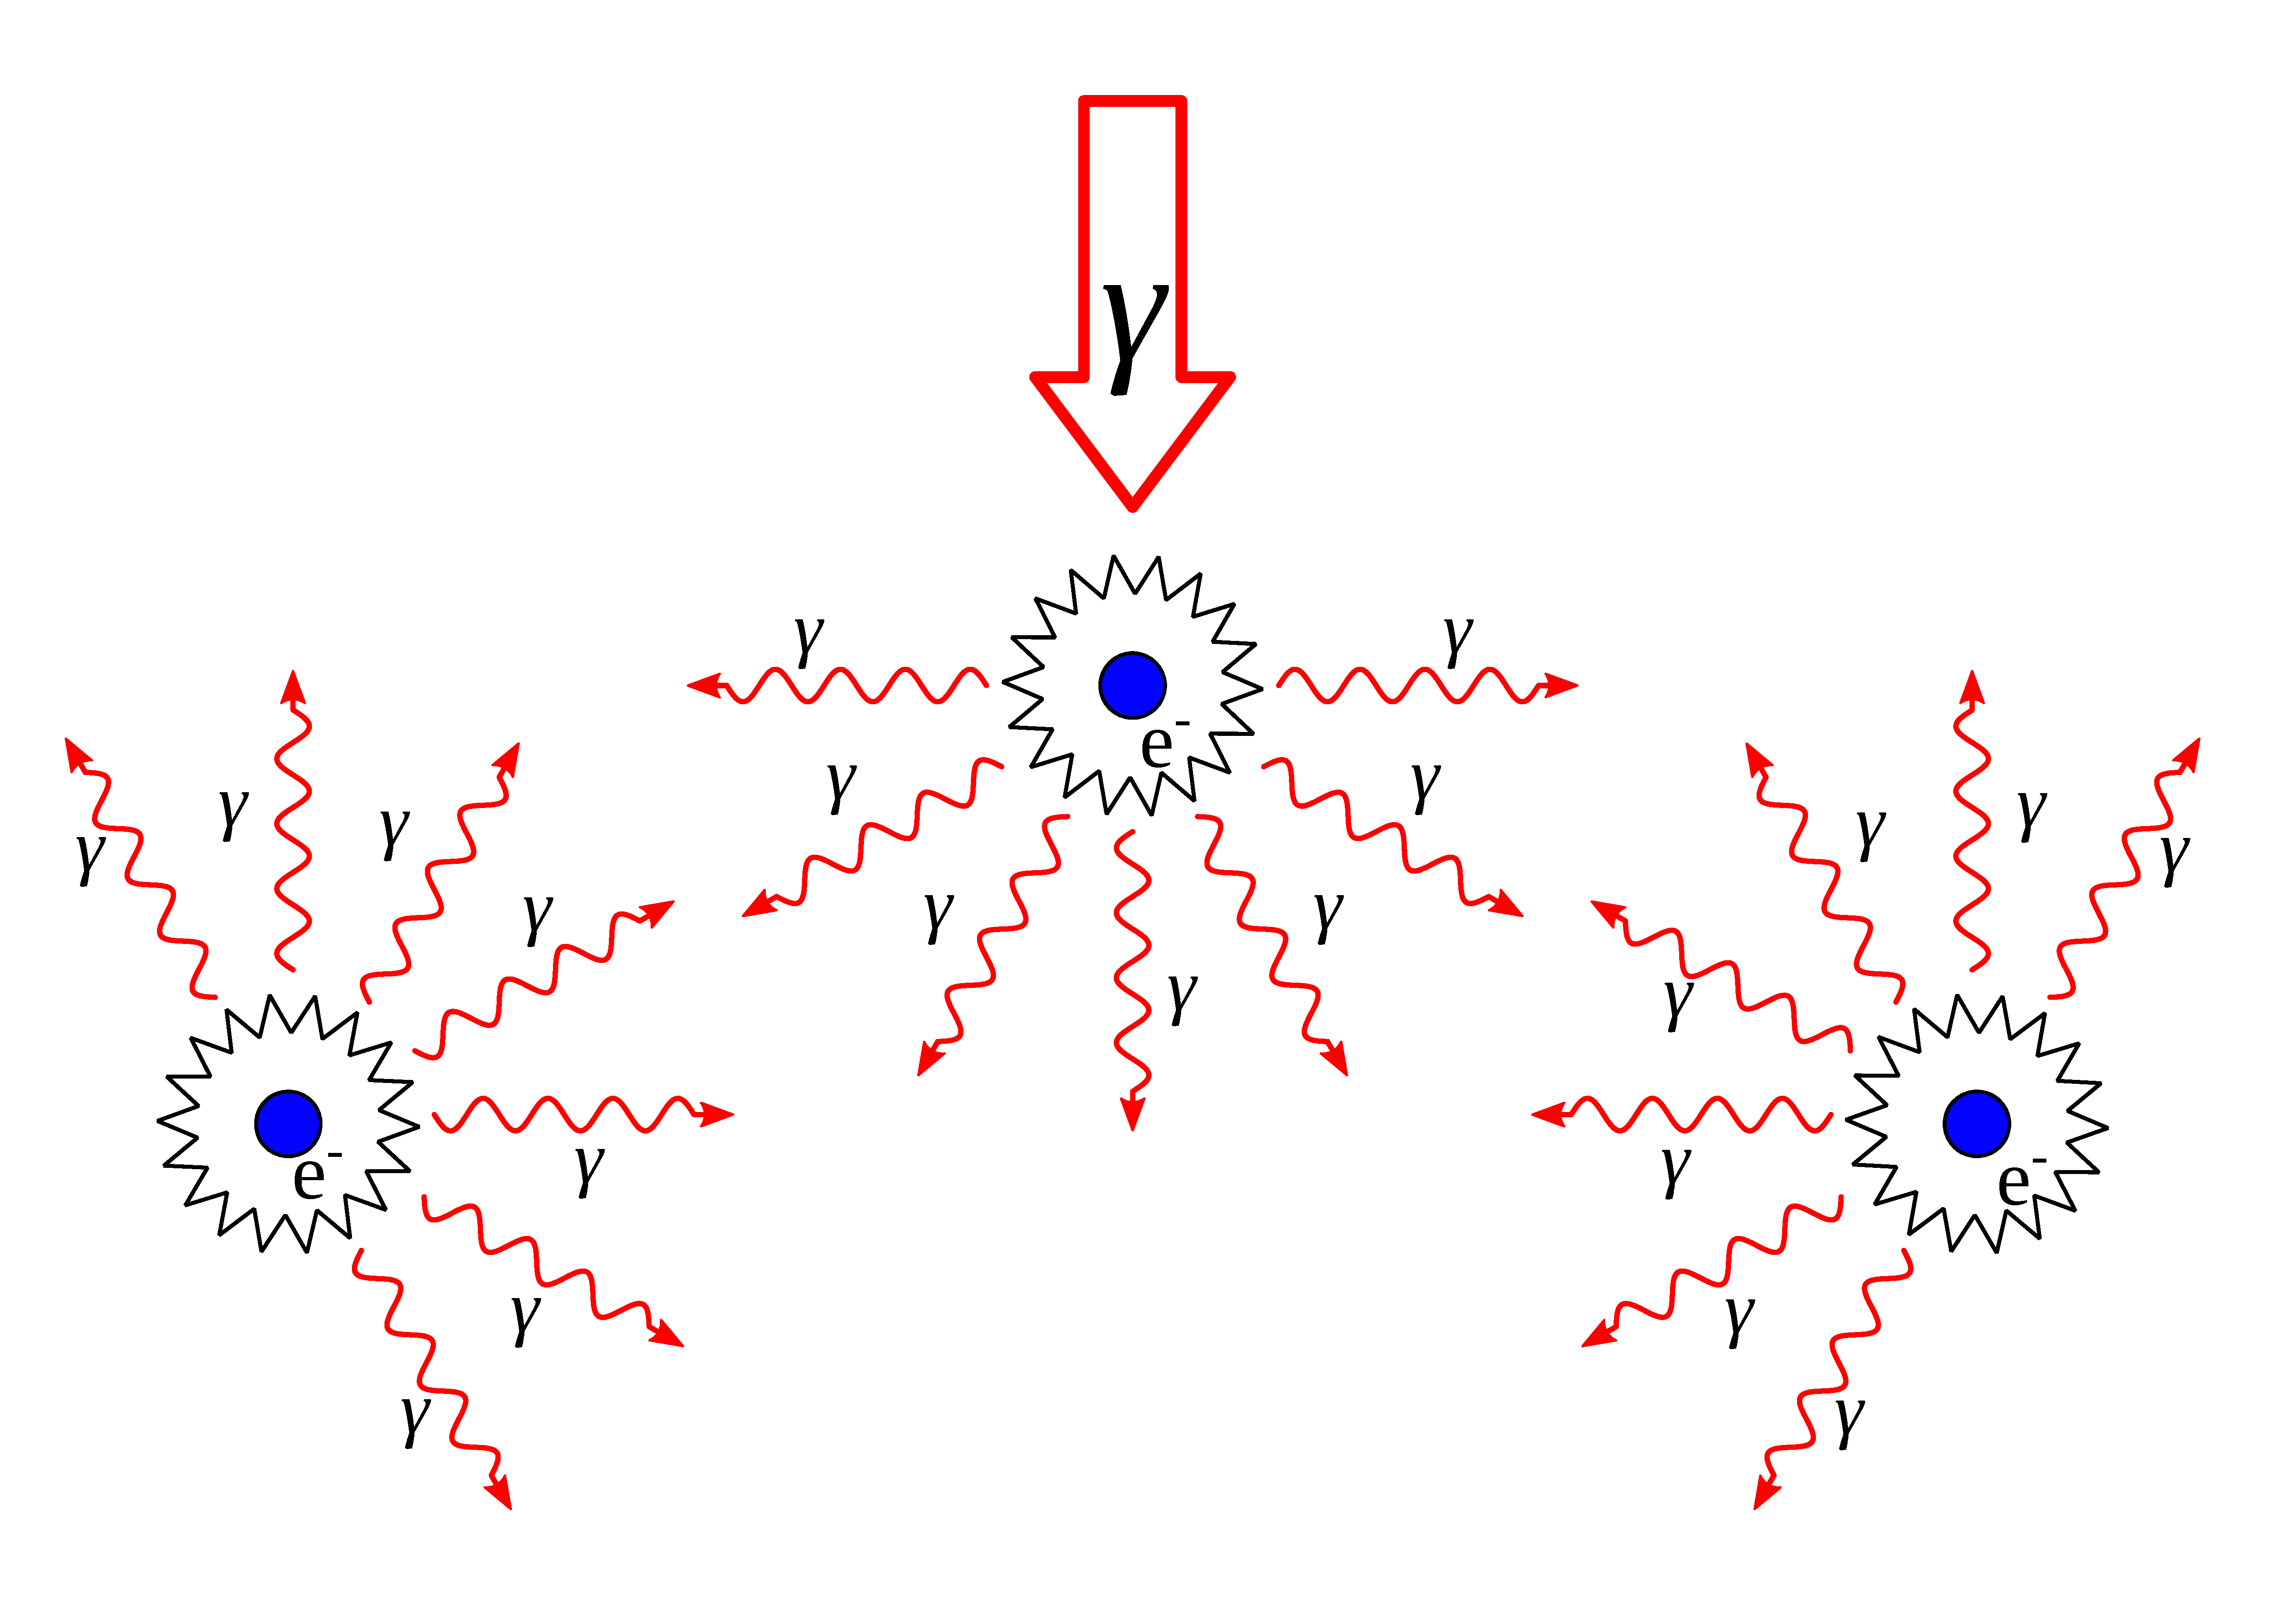
\includegraphics[width=0.8\paperwidth]{draw.pdf}

\end{frame}
\usebackgroundtemplate{}
%\begin{frame}
%\frametitle{Reactor Like TGE model}
%
%\end{frame}


\begin{frame}
    \frametitle{Proof of concept}
   	For fast checking the potential of our idea, we considered a next simplified model:  
    \begin{itemize}
    	\item There are only one tuning parameter  --- the local coefficient of gamma multiplication, describing usefulness of atmosphere for generating secondary particles;
    	\item Production of Gamma in cell occurs by Poisson distribution, momentum direction of generated gamma is defined by the electric field direction;
    	\item Electric field is chaotic: in point of cell ignition, direction of field is generated by uniform distribution, but magnitudes is constant for whole cloud;
    	\item Energy of particle not taken into account, propagation of gamma simulated with exponential distribution with fixed mean free path;
    	\item Cloud size is equals 1 kilometer and tracking of particle leaving volume stopped. 
    \end{itemize}
    This model is implemented as program on Kotlin programming language.
    
    
\end{frame}

\begin{frame}
    \frametitle{Results}
\begin{columns}
	\begin{column}{0.5\textwidth}
		\begin{figure}[htb]
		\centering
		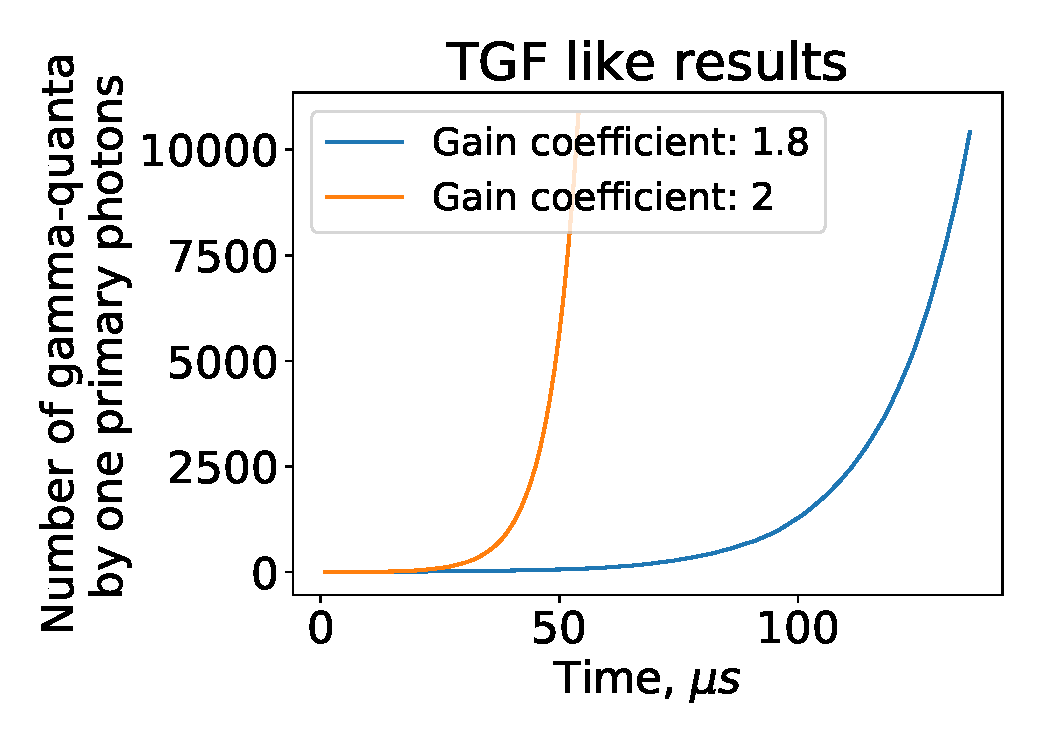
\includegraphics[width=1\columnwidth]{proofTGF.pdf}
		\end{figure}
		This figure shows the case of an \textbf{explosive growth} in the number of secondary photons that are well suited to the phenomenon of \textbf{TGF}.
	\end{column}
	\begin{column}{0.5\textwidth}
		\begin{figure}[htb]
			\centering
			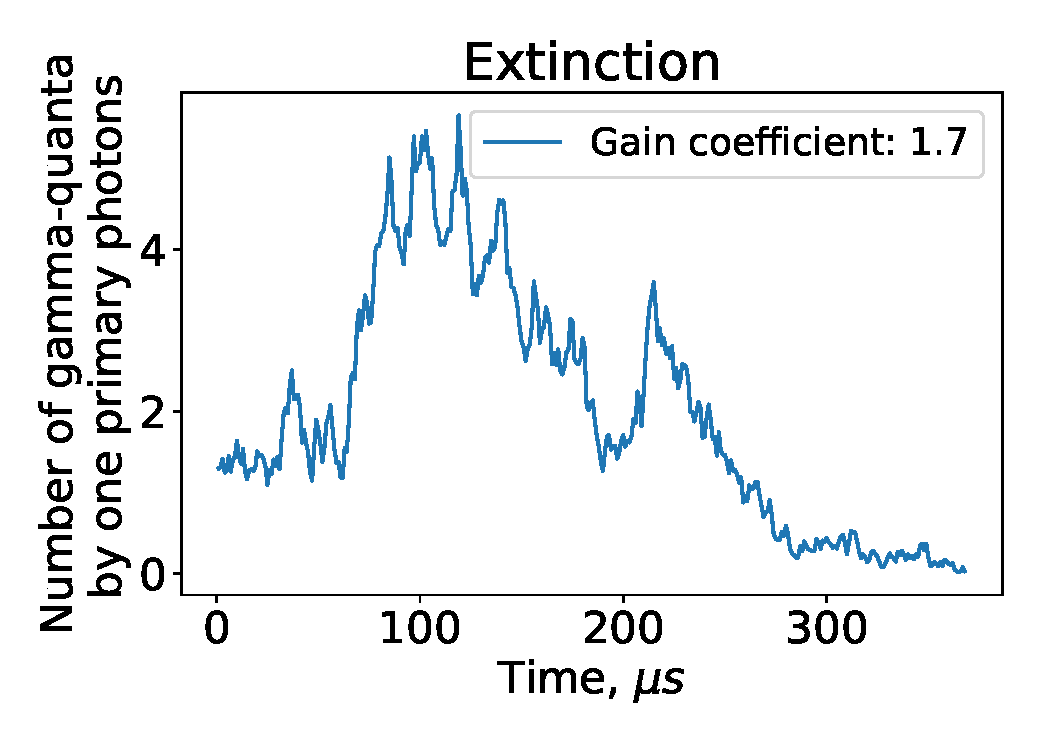
\includegraphics[width=1\columnwidth]{Extinction.pdf}
		\end{figure}
		This figure demonstrates the case when there was a \textbf{dissipation of an avalanche} that had just begun to develop.

	\end{column}
\end{columns}
    
\end{frame}


\begin{frame}
    \frametitle{Results}
    
    \begin{columns}
    	
    	\begin{column}{0.5\textwidth}
    		
    		\begin{figure}[htb]
    			\centering
    			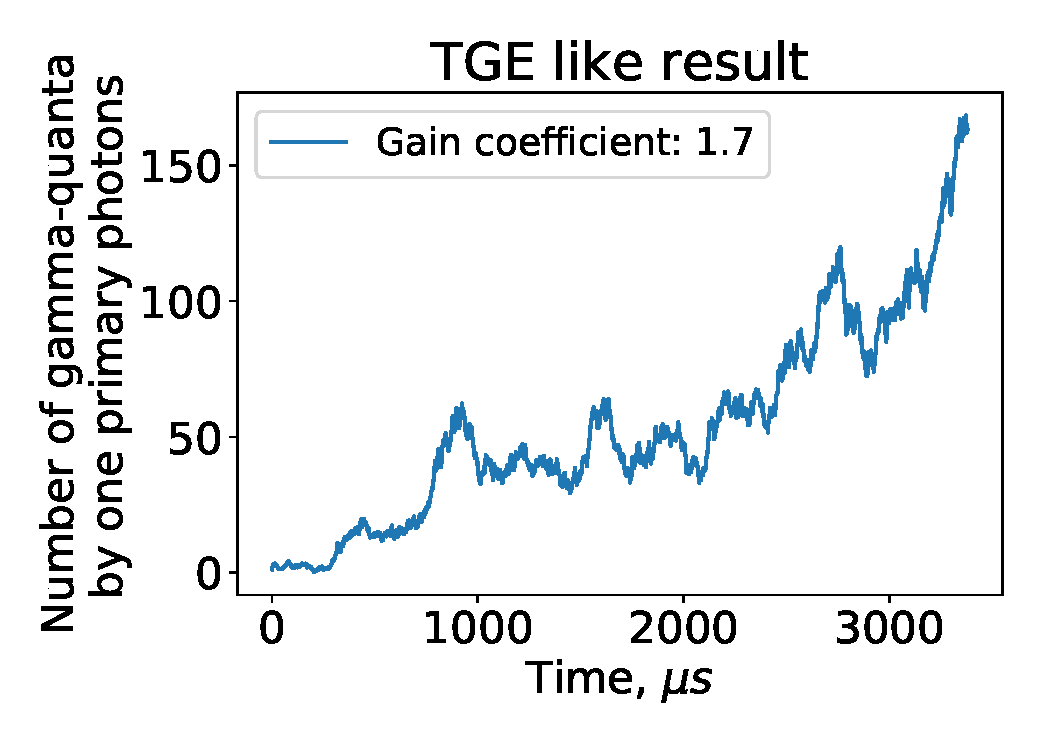
\includegraphics[width=1\columnwidth]{proofTGE.pdf}
    		\end{figure}
    		This figure demonstrates the case of a \textbf{slower and less intensive growth}. Such processes with some minor adjustments and assumptions about field dynamics could describe \textbf{TGE} phenomenon.	
    	\end{column}
    \end{columns}

\end{frame}


\begin{frame}
\frametitle{Conclusion}
				\begin{itemize}
	\item Reactor-like model is very good to describe TGF and other fast processes;
	\item Slow processes like TGE could be described with additional assumptions about field dynamics;
	\item The model could describe both TGE and TGF with the same mechanism depending on the state of the cloud.
\end{itemize}
Also reactor like model give next experimentally verifiable consequences:
\begin{itemize}
	\item Contrary to Dwyer and unmodified Gurevitch models, reactor model predicts quasi-isotropic (according to field distribution) emmittance of gamma-rays from a thundercloud.
	
	Measurement of the angular distribution of gamma-rays is required to prove or disprove the concept
	
	\item At first approximation, the energy spectrum of photons produced in RL model does not depend on radiation intensity (the spectrum depends on cell field and intensity on cell number).
\end{itemize}
Moreover reactor like TGE model can be used to investigate intercloud interaction.
\end{frame}

\begin{frame}
\frametitle{Thank you for your attention}

\end{frame}


\begin{frame}
\frametitle{Improved model}
\begin{columns}
	\begin{column}{0.45\textwidth}
               Our simple implementation of reactor like model show potential possibility, but its use a mean value of parameter. 
Improved model clarify  rough approximations of simple model, namely:
\begin{itemize}
	\item For generating electric field map used fractal model.
	\item The photons cross-section and energy-angular distribution sampling  is computed exactly, for tracking used algorithm of maximal cross-section;
	\item The spectrum of secondary particle from burned cell is simulated by GEANT4.
	
\end{itemize}
	\end{column}
	\begin{column}{0.45\textwidth}
            Also we improved output simulation information and made calculation is parallel.
By now we conduct only first simulation with improved model and we can only say, what conclusion received from simple model  haves been confirmed. For example on this figure shows evolution of  number of relativistic electron for small time interval.
\begin{figure}[htb]
	\centering
	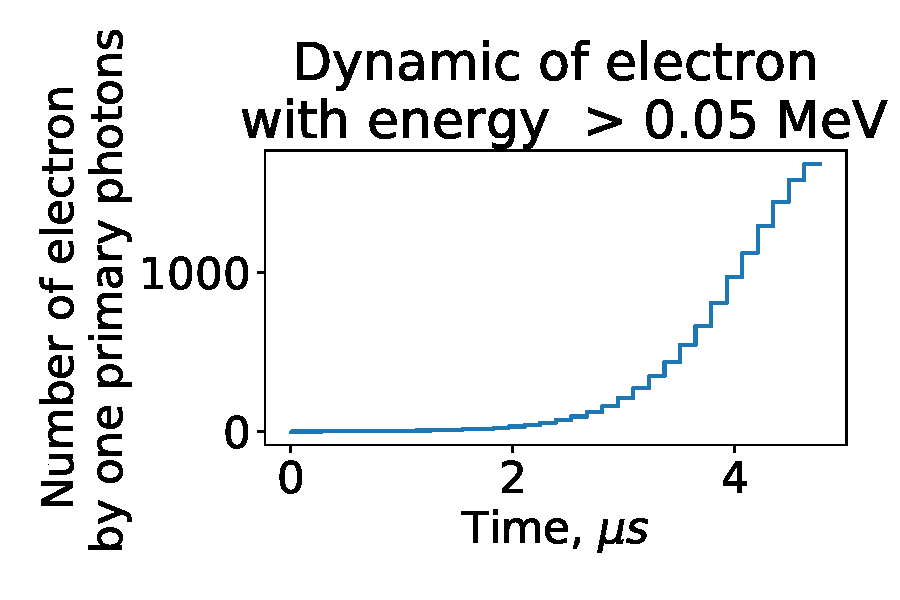
\includegraphics[width=1\columnwidth]{kotlinElectron.pdf}
	
\end{figure}
		
	\end{column}
\end{columns}
\end{frame}


\end{document}